\section{Supplementary Material} \label{SuppM}
\subsection*{Visual Learning Sequence Paradigm}
\begin{table}[H]
\centering
\begin{tabular}{lccccc}
\hline
            & \textbf{Repetition 1} & \textbf{Repetition 2} & \textbf{Repetition 3} & \textbf{Repetition 4} & \textbf{Repetition 5} \\ \hline
\textbf{UN} & 7'759                 & 5'378                 & 4'560                 & 4'005                 & 3'598                 \\
\textbf{NL} & 4'913                 & 2'174                 & 1'964                 & 1'779                 & 1'692                 \\
\textbf{K}  & 0                     & 3'092                 & 3'528                 & 3'864                 & 4'137                 \\
\textbf{F}  & 0                     & 1'543                 & 1'409                 & 1'369                 & 1'297                 \\ \hline
\end{tabular}
\caption[]{Total Learning Categories per Repetitions.}
\label{tab:RepLC}
\end{table}

\begin{table}[H]
\centering
\begin{tabular}{lcccccc}
\hline
\multicolumn{2}{c}{\textbf{Trials}}                & \multicolumn{5}{c}{\textbf{Learning Categories}}                     \\ \hline
               & \textbf{Mean Trials/Subject (SD)} & \textbf{Total} & \textbf{UN} & \textbf{NL} & \textbf{K} & \textbf{F} \\ \cline{2-7} 
\textbf{S7}    & 27.42 (4.61)                      & 14'833         & 6'263       & 3'268       & 3'821      & 1'481      \\
\textbf{S10}   & 41.05 (6.95)                      & 43'227         & 19'037      & 9'254       & 10'799     & 4'137      \\
\textbf{Total} & 36.42 (8.99)                      & 58'060         & 25'300      & 12'522      & 14'620     & 5'618      \\ \hline 
\multicolumn{7}{l}{\small \textit{Note.} UN = Unknown, NL = Newly Learned, K = Known, F = Forgotten.}
\end{tabular}
\caption[]{Summary of Trials and Learning Categories}
\label{tab:my_label}
\end{table}

\begin{table}[H]
\centering
\begin{tabular}{lcllllll}
\hline
                           & \multicolumn{7}{c}{\textbf{Age Groups (years):}}                                                                                                                                              \\ 
                           & \multicolumn{1}{l}{\textbf{5-7}} & \textbf{7-9}            & \textbf{9-11}           & \textbf{11-13}          & \textbf{13-15}          & \textbf{15-17}          & \textbf{17-22}          \\\cline{2-8} 
\textbf{Peak Latency (ms)} & 454                              & \multicolumn{1}{c}{422} & \multicolumn{1}{c}{412} & \multicolumn{1}{c}{400} & \multicolumn{1}{c}{414} & \multicolumn{1}{c}{398} & \multicolumn{1}{c}{392} \\ \hline
\end{tabular}
\caption[]{P300 Peak Latency of Age Groups}
\label{tab:peaklatency}

\end{table}


\newpage
\begin{figure}[H]
    \centering
    \includegraphics[width=0.8\linewidth]{Subfigures/topoall.png}
    \caption[]{Topoplots for Electrodes Selection.}
    \label{fig:elecsel}
\end{figure}

\newpage
\subsection*{Why Different Knowledge Index} \label{chap:stein}
Figure \ref{fig:steine} visualizes the study design in \textcite{steinemannTrackingNeuralCorrelates2016} paper. Since learning categories were created by comparing pre and posttest, the possibilty that a given stimulus location categorized as newly learned (i.e., pretest incorrect and posttest correct) could actually become known (i.e., twice correct) during the three sequence presentations led the authors to weight the newly learned learning categories with 0.5. In this thesis, behavior response is acquired after every sequence, therefore, the newly learned categories were not weighted. 
\begin{figure}[H]
\centering
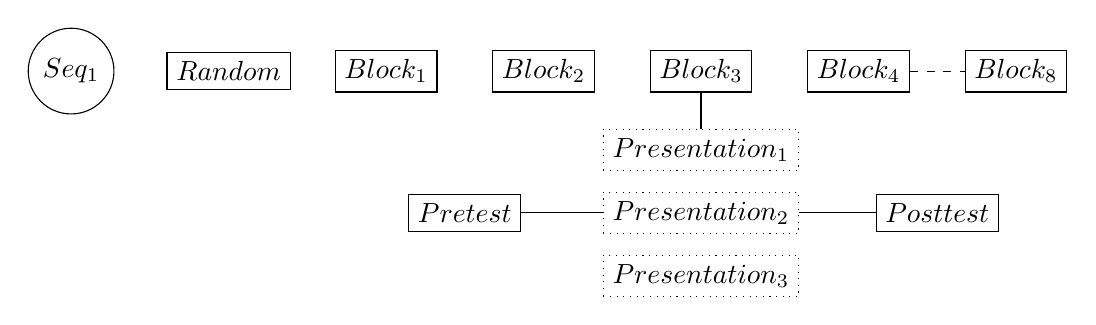
\begin{tikzpicture}
        \node at (0,0)[circle,draw] (c100)  {$Seq_1$};
        \node at (2,0) [rectangle,draw] (c200) {$Random$};
        \node at (4,0) [rectangle,draw] (c300) {$Block_1$};
        
         \node at (8,-2.6) [rectangle,draw,dotted] (c170) {$Presentation_3$};
        \node at (8,-1.8) [rectangle,draw,dotted] (c160) {$Presentation_2$};
         \node at (8,-1) [rectangle,draw,dotted] (c150) {$Presentation_1$};
        \node at (5,-1.8) [rectangle,draw] (c110) {$Pre test$};
        \node at (11,-1.8) [rectangle,draw] (c120) {$Post test$}; 
         \draw (c120)--(c160);
        \draw (c110)--(c160);

       \node at (6,0) [rectangle,draw] (c400) {$Block_2$};
        \node at (8,0) [rectangle,draw] (c500) {$Block_3$};
        \node at (10,0) [rectangle,draw] (c600) {$Block_4$};
       \node at (12,0) [rectangle,draw] (c700) {$Block_8$};
        \draw (c500)--(c150);
       \draw[dashed] (c600)--(c700);
      
    \end{tikzpicture}
\caption[]{Study design of experiement 2 in \textcite{steinemannTrackingNeuralCorrelates2016} visualized for the first sequence.} \label{fig:steine}
\end{figure}
\newpage
\subsection*{Network Analysis}
\begin{figure}[H]
    \centering
    \includegraphics[width=0.8\linewidth]{Subfigures/Expl_dist_pre_trans.jpeg}
    \caption[]{Distribution of Variables included in the Network Analysis.}
    \label{fig:distall}
\end{figure}


\begin{figure}[H]
    \centering
    \includegraphics[width=0.6\linewidth]{Subfigures/Posttransform.jpeg}
    \caption[]{Distribution of Variables transformed. A: Before transformation. B: After transformation.}
    \label{fig:distaftert}
\end{figure}

\begin{table}[H]
\centering
\begin{tabular}{ccccccccccccc}
\hline
             & \textbf{V1} & \textbf{V2} & \textbf{V3} & \textbf{V4} & \textbf{V5} & \textbf{V6} & \textbf{V7} & \textbf{V8} & \textbf{V9} & \textbf{V10} & \textbf{V11} & \textbf{V12} \\ \hline
\textbf{V1}  &             &             &             &             &             &             &             &             &             &              &              &              \\
\textbf{V2}  & 0.30        &             &             &             &             &             &             &             &             &              &              &              \\
\textbf{V3}  & 0.48        & 0.09        &             &             &             &             &             &             &             &              &              &              \\
\textbf{V4}  & 0.08        & 0.00        & 0.00        &             &             &             &             &             &             &              &              &              \\
\textbf{V5}  & 0.00        & 0.00        & 0.00        & 0.35        &             &             &             &             &             &              &              &              \\
\textbf{V6}  & 0.00        & 0.00        & 0.00        & -0.25       & 0.00        &             &             &             &             &              &              &              \\
\textbf{V7}  & -0.18       & 0.17        & 0.10        & 0.00        & -0.19       & 0.00        &             &             &             &              &              &              \\
\textbf{V8}  & 0.00        & 0.00        & 0.00        & 0.23        & 0.18        & 0.00        & 0.21        &             &             &              &              &              \\
\textbf{V9}  & 0.00        & 0.00        & 0.00        & 0.07        & 0.00        & 0.00        & 0.00        & -0.07       &             &              &              &              \\
\textbf{V10} & 0.00        & 0.41        & -0.15       & 0.00        & 0.00        & 0.00        & 0.00        & 0.00        & 0.00        &              &              &              \\
\textbf{V11} & 0.14        & -0.08       & 0.23        & -0.09       & 0.00        & 0.00        & 0.00        & 0.00        & 0.00        & 0.00         &              &              \\
\textbf{V12} & 0.40        & -0.09       & -0.11       & 0.00        & -0.12       & 0.11        & 0.08        & -0.07       & 0.00        & 0.17         & 0.00         &              \\ \hline
\end{tabular}
\caption[]{Partical Correlation Matrix (estimated with ggmModSelect).}
\label{tab:parcorrm}
\end{table}

\begin{table}[]
\centering
\begin{tabular}{lllllllllllll}
\hline
\textbf{Nodes}                & \textbf{V1} & \textbf{V2} & \textbf{V3} & \textbf{V4} & \textbf{V5} & \textbf{V6} & \textbf{V7} & \textbf{V8} & \textbf{V9} & \textbf{V10} & \textbf{V11} & \textbf{V12} \\ \hline
\textbf{$R^2$} & 0.65        & 0.52        & 0.48        & 0.30        & 0.26        & 0.11        & 0.13        & 0.18        & 0.01        & 0.71         & 0.73         & 0.35         \\ \hline
\end{tabular}
\caption[]{Explained Variance of each Node in Network Analysis.}
\label{tab:Rsqu}
\end{table}






